\documentclass[12pt]{article}
\usepackage{commands}



\begin{document}









 \begin{tikzpicture}[remember picture,overlay]
         % If a chapter image has been specified
%         \expandafter\ifstrequal\expandafter{Images/vendingMachine.png}{}{}{
	                 % Output the chapter image
	                 \node[
	                 anchor=north west, % Anchor point on the image
	                 inner sep=0pt, % Inner padding
	                 ] at (current page.north west) {\includegraphics[angle=0,height=\paperheight]{Images/vendingMachine.png}};
%	         }
 \end{tikzpicture} 
 
  
  \vspace{-1.8cm}
\heading{How to Make a Coffee Vending Machine Using Dynamical Systems!}


\newpage

\section{Introduction}
This a an informal writing to share some ridiculous thoughts on making a vending using dynamical systems! I know this is a very inaccurate title, but what I really mean is to utilize the hysteresis mechanism that appears in some dynamical systems to design a very simple finite automate, from which we can easily design a simple vending machine.   


\section{Hysteresis in Dynamical Systems}
Some dynamical systems has a kind of ``memory'' or ``hysteresis'', in which the change in the state of the system in the bifurcation point depends on the specific direction that we approach the critical value for bifurcation. Although we can come up with much more simpler systems who admits hysteresis, here I am actually going to consider the following system
\[ \dot{x}= rx + x^3 - x^5, \]
where $\dot{x}$ means the time derivative of $x\in \R$, and $r\in\R$\ is a constant. By doing the bifurcation analysis on this particular system, we soon find out that the system has a pitchfork bifurcation and its bifurcation diagram is something like the following figure.
\begin{figure}[h!]
	\centering
	
	
	
	
	\tikzset{every picture/.style={line width=0.75pt}} %set default line width to 0.75pt        
	
	\begin{tikzpicture}[x=0.75pt,y=0.75pt,yscale=-1.5,xscale=1.5]
		%uncomment if require: \path (0,300); %set diagram left start at 0, and has height of 300
		
		%Curve Lines [id:da3475967864092384] 
		\draw    (330,60) .. controls (309.5,60) and (240,70) .. (240,90) .. controls (240,110) and (280.5,107.5) .. (280,120) .. controls (279.5,132.5) and (239.5,129.5) .. (240,150) .. controls (240.5,170.5) and (312,179) .. (330,180) ;
		%Straight Lines [id:da8628159498522963] 
		\draw    (190,120) -- (280,120) ;
		%Straight Lines [id:da07087007695378178] 
		\draw  [dash pattern={on 4.5pt off 4.5pt}]  (280,120) -- (330,120) ;
		%Straight Lines [id:da9630925968212913] 
		\draw [color={rgb, 255:red, 255; green, 255; blue, 255 }  ,draw opacity=1 ][line width=3]    (240,89.67) -- (241.33,95.33) ;
		%Straight Lines [id:da10933997251577554] 
		\draw [color={rgb, 255:red, 255; green, 255; blue, 255 }  ,draw opacity=1 ][line width=3]    (243.33,98.33) -- (248,103) ;
		%Straight Lines [id:da39451280789014165] 
		\draw [color={rgb, 255:red, 255; green, 255; blue, 255 }  ,draw opacity=1 ][line width=3]    (252.33,104.67) -- (257.67,106.67) ;
		%Straight Lines [id:da7877273412409396] 
		\draw [color={rgb, 255:red, 255; green, 255; blue, 255 }  ,draw opacity=1 ][line width=3]    (262,108.67) -- (267.33,110.67) ;
		%Straight Lines [id:da949863006732423] 
		\draw [color={rgb, 255:red, 255; green, 255; blue, 255 }  ,draw opacity=1 ][line width=3]    (272.33,112.33) -- (277.67,114.33) ;
		%Straight Lines [id:da6008132146686285] 
		\draw [color={rgb, 255:red, 255; green, 255; blue, 255 }  ,draw opacity=1 ][line width=3]    (275,127.33) -- (278.67,123.67) ;
		%Straight Lines [id:da6428214676220647] 
		\draw [color={rgb, 255:red, 255; green, 255; blue, 255 }  ,draw opacity=1 ][line width=3]    (264.67,131) -- (270.67,128.33) ;
		%Straight Lines [id:da557059542843994] 
		\draw [color={rgb, 255:red, 255; green, 255; blue, 255 }  ,draw opacity=1 ][line width=3]    (254.67,134.33) -- (260.67,131.67) ;
		%Straight Lines [id:da14327656158346214] 
		\draw [color={rgb, 255:red, 255; green, 255; blue, 255 }  ,draw opacity=1 ][line width=3]    (244.33,138.67) -- (250.33,136) ;
		%Straight Lines [id:da5660831756940781] 
		\draw [color={rgb, 255:red, 255; green, 255; blue, 255 }  ,draw opacity=1 ][line width=3]    (239.33,147.33) -- (242.33,142) ;
		%Straight Lines [id:da3939017840273582] 
		\draw [color={rgb, 255:red, 255; green, 0; blue, 0 }  ,draw opacity=1 ]   (186,77) -- (203,77) ;
		\draw [shift={(206,77)}, rotate = 180] [fill={rgb, 255:red, 255; green, 0; blue, 0 }  ,fill opacity=1 ][line width=0.08]  [draw opacity=0] (7.14,-3.43) -- (0,0) -- (7.14,3.43) -- (4.74,0) -- cycle    ;
		%Straight Lines [id:da4292502511319951] 
		\draw [color={rgb, 255:red, 255; green, 0; blue, 0 }  ,draw opacity=1 ]   (186,77) -- (186,60) ;
		\draw [shift={(186,57)}, rotate = 90] [fill={rgb, 255:red, 255; green, 0; blue, 0 }  ,fill opacity=1 ][line width=0.08]  [draw opacity=0] (7.14,-3.43) -- (0,0) -- (7.14,3.43) -- (4.74,0) -- cycle    ;
		
		% Text Node
		\draw (207,76) node [anchor=north west][inner sep=0.75pt]  [font=\scriptsize,xscale=2,yscale=2] [align=left] {$\displaystyle r$};
		% Text Node
		\draw (173.67,47) node [anchor=north west][inner sep=0.75pt]  [font=\scriptsize,xscale=2,yscale=2] [align=left] {$\displaystyle \hat{x}$};
		% Text Node
		\draw (280.33,125.33) node [anchor=north west][inner sep=0.75pt]  [font=\scriptsize,xscale=2,yscale=2] [align=left] {0};
		
		
	\end{tikzpicture}
\end{figure}

As we can see from the figure above, this system admits stable and unstable steady states for different values of the control parameter $r$. However, the interesting point for us here is the hysteresis mechanism that is hidden in the bifurcation diagram. The following figure makes this more clear. 

\begin{figure}[h!]
	\centering
	
	
	\tikzset{every picture/.style={line width=0.75pt}} %set default line width to 0.75pt        
	
	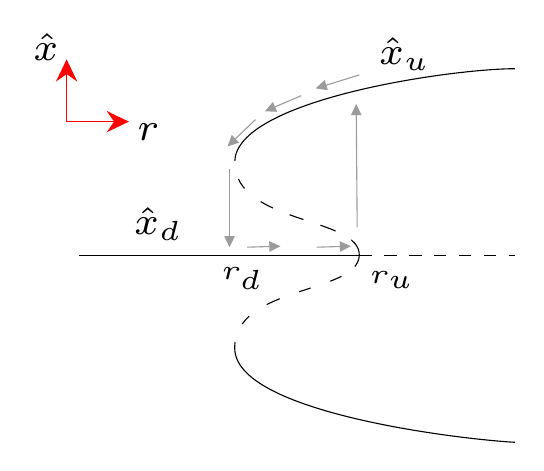
\begin{tikzpicture}[x=0.75pt,y=0.75pt,yscale=-1.5,xscale=1.5]
		%uncomment if require: \path (0,300); %set diagram left start at 0, and has height of 300
		
		%Curve Lines [id:da3475967864092384] 
		\draw    (330,60) .. controls (309.5,60) and (240,70) .. (240,90) .. controls (240,110) and (280.5,107.5) .. (280,120) .. controls (279.5,132.5) and (239.5,129.5) .. (240,150) .. controls (240.5,170.5) and (312,179) .. (330,180) ;
		%Straight Lines [id:da8628159498522963] 
		\draw    (190,120) -- (280,120) ;
		%Straight Lines [id:da07087007695378178] 
		\draw  [dash pattern={on 4.5pt off 4.5pt}]  (280,120) -- (330,120) ;
		%Straight Lines [id:da9630925968212913] 
		\draw [color={rgb, 255:red, 255; green, 255; blue, 255 }  ,draw opacity=1 ][line width=3]    (240,89.67) -- (241.33,95.33) ;
		%Straight Lines [id:da10933997251577554] 
		\draw [color={rgb, 255:red, 255; green, 255; blue, 255 }  ,draw opacity=1 ][line width=3]    (243.33,98.33) -- (248,103) ;
		%Straight Lines [id:da39451280789014165] 
		\draw [color={rgb, 255:red, 255; green, 255; blue, 255 }  ,draw opacity=1 ][line width=3]    (252.33,104.67) -- (257.67,106.67) ;
		%Straight Lines [id:da7877273412409396] 
		\draw [color={rgb, 255:red, 255; green, 255; blue, 255 }  ,draw opacity=1 ][line width=3]    (262,108.67) -- (267.33,110.67) ;
		%Straight Lines [id:da949863006732423] 
		\draw [color={rgb, 255:red, 255; green, 255; blue, 255 }  ,draw opacity=1 ][line width=3]    (272.33,112.33) -- (277.67,114.33) ;
		%Straight Lines [id:da6008132146686285] 
		\draw [color={rgb, 255:red, 255; green, 255; blue, 255 }  ,draw opacity=1 ][line width=3]    (275,127.33) -- (278.67,123.67) ;
		%Straight Lines [id:da6428214676220647] 
		\draw [color={rgb, 255:red, 255; green, 255; blue, 255 }  ,draw opacity=1 ][line width=3]    (264.67,131) -- (270.67,128.33) ;
		%Straight Lines [id:da557059542843994] 
		\draw [color={rgb, 255:red, 255; green, 255; blue, 255 }  ,draw opacity=1 ][line width=3]    (254.67,134.33) -- (260.67,131.67) ;
		%Straight Lines [id:da14327656158346214] 
		\draw [color={rgb, 255:red, 255; green, 255; blue, 255 }  ,draw opacity=1 ][line width=3]    (244.33,138.67) -- (250.33,136) ;
		%Straight Lines [id:da5660831756940781] 
		\draw [color={rgb, 255:red, 255; green, 255; blue, 255 }  ,draw opacity=1 ][line width=3]    (239.33,147.33) -- (242.33,142) ;
		%Straight Lines [id:da3939017840273582] 
		\draw [color={rgb, 255:red, 255; green, 0; blue, 0 }  ,draw opacity=1 ]   (186,77) -- (203,77) ;
		\draw [shift={(206,77)}, rotate = 180] [fill={rgb, 255:red, 255; green, 0; blue, 0 }  ,fill opacity=1 ][line width=0.08]  [draw opacity=0] (7.14,-3.43) -- (0,0) -- (7.14,3.43) -- (4.74,0) -- cycle    ;
		%Straight Lines [id:da4292502511319951] 
		\draw [color={rgb, 255:red, 255; green, 0; blue, 0 }  ,draw opacity=1 ]   (186,77) -- (186,60) ;
		\draw [shift={(186,57)}, rotate = 90] [fill={rgb, 255:red, 255; green, 0; blue, 0 }  ,fill opacity=1 ][line width=0.08]  [draw opacity=0] (7.14,-3.43) -- (0,0) -- (7.14,3.43) -- (4.74,0) -- cycle    ;
		%Straight Lines [id:da04468453728060462] 
		\draw [color={rgb, 255:red, 155; green, 155; blue, 155 }  ,draw opacity=1 ]   (268.87,65.45) -- (280,62) ;
		\draw [shift={(266,66.33)}, rotate = 342.8] [fill={rgb, 255:red, 155; green, 155; blue, 155 }  ,fill opacity=1 ][line width=0.08]  [draw opacity=0] (3.57,-1.72) -- (0,0) -- (3.57,1.72) -- cycle    ;
		%Straight Lines [id:da6421999189293346] 
		\draw [color={rgb, 255:red, 155; green, 155; blue, 155 }  ,draw opacity=1 ]   (252.42,72.48) -- (261.33,68.67) ;
		\draw [shift={(249.67,73.67)}, rotate = 336.8] [fill={rgb, 255:red, 155; green, 155; blue, 155 }  ,fill opacity=1 ][line width=0.08]  [draw opacity=0] (3.57,-1.72) -- (0,0) -- (3.57,1.72) -- cycle    ;
		%Straight Lines [id:da3913600379521629] 
		\draw [color={rgb, 255:red, 155; green, 155; blue, 155 }  ,draw opacity=1 ]   (239.83,82.92) -- (246.67,76.33) ;
		\draw [shift={(237.67,85)}, rotate = 316.08] [fill={rgb, 255:red, 155; green, 155; blue, 155 }  ,fill opacity=1 ][line width=0.08]  [draw opacity=0] (3.57,-1.72) -- (0,0) -- (3.57,1.72) -- cycle    ;
		%Straight Lines [id:da2959398371731523] 
		\draw [color={rgb, 255:red, 155; green, 155; blue, 155 }  ,draw opacity=1 ]   (238.33,114.33) -- (238.33,92.33) ;
		\draw [shift={(238.33,117.33)}, rotate = 270] [fill={rgb, 255:red, 155; green, 155; blue, 155 }  ,fill opacity=1 ][line width=0.08]  [draw opacity=0] (3.57,-1.72) -- (0,0) -- (3.57,1.72) -- cycle    ;
		%Straight Lines [id:da6212681777845439] 
		\draw [color={rgb, 255:red, 155; green, 155; blue, 155 }  ,draw opacity=1 ]   (251.67,117.09) -- (244,117.33) ;
		\draw [shift={(254.67,117)}, rotate = 178.21] [fill={rgb, 255:red, 155; green, 155; blue, 155 }  ,fill opacity=1 ][line width=0.08]  [draw opacity=0] (3.57,-1.72) -- (0,0) -- (3.57,1.72) -- cycle    ;
		%Straight Lines [id:da8168119094171771] 
		\draw [color={rgb, 255:red, 155; green, 155; blue, 155 }  ,draw opacity=1 ]   (274.33,117.09) -- (266.33,117.33) ;
		\draw [shift={(277.33,117)}, rotate = 178.26] [fill={rgb, 255:red, 155; green, 155; blue, 155 }  ,fill opacity=1 ][line width=0.08]  [draw opacity=0] (3.57,-1.72) -- (0,0) -- (3.57,1.72) -- cycle    ;
		%Straight Lines [id:da604904148477025] 
		\draw [color={rgb, 255:red, 155; green, 155; blue, 155 }  ,draw opacity=1 ]   (279.03,74.33) -- (279.33,111) ;
		\draw [shift={(279,71.33)}, rotate = 89.52] [fill={rgb, 255:red, 155; green, 155; blue, 155 }  ,fill opacity=1 ][line width=0.08]  [draw opacity=0] (3.57,-1.72) -- (0,0) -- (3.57,1.72) -- cycle    ;
		
		% Text Node
		\draw (207,76) node [anchor=north west][inner sep=0.75pt]  [font=\scriptsize,xscale=2,yscale=2] [align=left] {$\displaystyle r$};
		% Text Node
		\draw (173.67,47) node [anchor=north west][inner sep=0.75pt]  [font=\scriptsize,xscale=2,yscale=2] [align=left] {$\displaystyle \hat{x}$};
		% Text Node
		\draw (234,122.33) node [anchor=north west][inner sep=0.75pt]  [font=\tiny,xscale=2,yscale=2] [align=left] {$\displaystyle r_{d}$};
		% Text Node
		\draw (281.67,123.33) node [anchor=north west][inner sep=0.75pt]  [font=\tiny,xscale=2,yscale=2] [align=left] {$\displaystyle r_{u}$};
		% Text Node
		\draw (206,103) node [anchor=north west][inner sep=0.75pt]  [font=\scriptsize,xscale=2,yscale=2] [align=left] {$\displaystyle \hat{x}_{d}$};
		% Text Node
		\draw (284.67,48.33) node [anchor=north west][inner sep=0.75pt]  [font=\scriptsize,xscale=2,yscale=2] [align=left] {$\displaystyle \hat{x}_{u}$};
		
		
	\end{tikzpicture}
\end{figure}

We call the upper branch of the stable steady state $\hat{x}_u$ (in which $u$ stands for up) and the middle branch of the stable steady state as $\hat{x}_d$ (in which $d$ stands for down). As we can trace on the diagram, starting with a steady state on the upper branch, and then decreasing the value of $r$, until we reach the bifurcation point at $r_d$, the state of the state suddenly jumps to $\hat{x}_d$, and it remains there for any sufficiently small perturbation around $r_d$. Then increasing the value of $r$, until we reach $r_u$ causes another jump in the steady state from the middle branch back to the upper branch. 

This phenomena is really similar to the finite state machine, where we have discrete states and the transition between states is governed by the system input. Also, as we have seen in the digital electronic, we can design systems that the transition in their state depends on the \emph{rising edge} or \emph{falling edge} of the signal, and the parallel here with that notion, is the specific way in which we approach the critical points. Consider the following finite state machine diagram for this system.
\begin{figure}[h!]
	\centering
	
	
	\tikzset{every picture/.style={line width=0.75pt}} %set default line width to 0.75pt        
	
	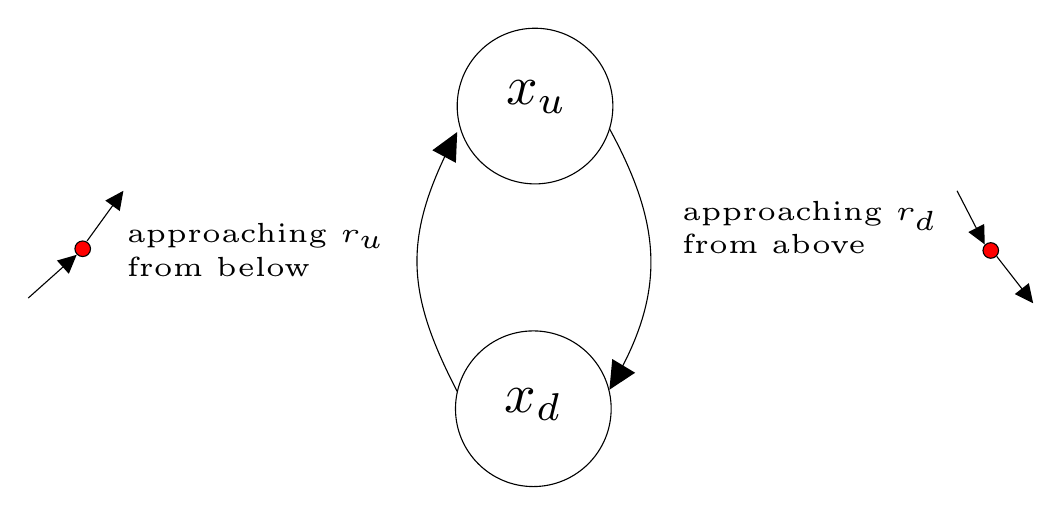
\begin{tikzpicture}[x=0.75pt,y=0.75pt,yscale=-2.5,xscale=2.5]
		%uncomment if require: \path (0,300); %set diagram left start at 0, and has height of 300
		
		%Shape: Circle [id:dp19444798196340818] 
		\draw   (180,45) .. controls (180,36.72) and (186.72,30) .. (195,30) .. controls (203.28,30) and (210,36.72) .. (210,45) .. controls (210,53.28) and (203.28,60) .. (195,60) .. controls (186.72,60) and (180,53.28) .. (180,45) -- cycle ;
		%Shape: Circle [id:dp816887625058681] 
		\draw   (179.67,103.33) .. controls (179.67,95.05) and (186.38,88.33) .. (194.67,88.33) .. controls (202.95,88.33) and (209.67,95.05) .. (209.67,103.33) .. controls (209.67,111.62) and (202.95,118.33) .. (194.67,118.33) .. controls (186.38,118.33) and (179.67,111.62) .. (179.67,103.33) -- cycle ;
		%Curve Lines [id:da5723668381117777] 
		\draw    (180,100) .. controls (170.45,81.54) and (169.41,70.98) .. (178.63,52.64) ;
		\draw [shift={(180,50)}, rotate = 118.07] [fill={rgb, 255:red, 0; green, 0; blue, 0 }  ][line width=0.08]  [draw opacity=0] (5.36,-2.57) -- (0,0) -- (5.36,2.57) -- cycle    ;
		%Curve Lines [id:da3010184020382227] 
		\draw    (210.9,96.96) .. controls (220.24,80.02) and (219.15,67.38) .. (209.33,49.33) ;
		\draw [shift={(209.33,99.67)}, rotate = 300.96] [fill={rgb, 255:red, 0; green, 0; blue, 0 }  ][line width=0.08]  [draw opacity=0] (5.36,-2.57) -- (0,0) -- (5.36,2.57) -- cycle    ;
		%Straight Lines [id:da3364125847880146] 
		\draw    (276.33,61.33) -- (280.29,69) ;
		\draw [shift={(281.67,71.67)}, rotate = 242.7] [fill={rgb, 255:red, 0; green, 0; blue, 0 }  ][line width=0.08]  [draw opacity=0] (3.57,-1.72) -- (0,0) -- (3.57,1.72) -- cycle    ;
		%Shape: Circle [id:dp801346546523267] 
		\draw  [fill={rgb, 255:red, 255; green, 0; blue, 0 }  ,fill opacity=1 ] (281.33,72.83) .. controls (281.33,72) and (282,71.33) .. (282.83,71.33) .. controls (283.66,71.33) and (284.33,72) .. (284.33,72.83) .. controls (284.33,73.66) and (283.66,74.33) .. (282.83,74.33) .. controls (282,74.33) and (281.33,73.66) .. (281.33,72.83) -- cycle ;
		%Straight Lines [id:da3400154107262219] 
		\draw    (284,74) -- (289.16,80.63) ;
		\draw [shift={(291,83)}, rotate = 232.13] [fill={rgb, 255:red, 0; green, 0; blue, 0 }  ][line width=0.08]  [draw opacity=0] (3.57,-1.72) -- (0,0) -- (3.57,1.72) -- cycle    ;
		%Straight Lines [id:da9364634936350018] 
		\draw    (97.33,82) -- (104.43,75.66) ;
		\draw [shift={(106.67,73.67)}, rotate = 138.24] [fill={rgb, 255:red, 0; green, 0; blue, 0 }  ][line width=0.08]  [draw opacity=0] (3.57,-1.72) -- (0,0) -- (3.57,1.72) -- cycle    ;
		%Shape: Circle [id:dp798299245137134] 
		\draw  [fill={rgb, 255:red, 255; green, 0; blue, 0 }  ,fill opacity=1 ] (106.33,72.5) .. controls (106.33,71.67) and (107,71) .. (107.83,71) .. controls (108.66,71) and (109.33,71.67) .. (109.33,72.5) .. controls (109.33,73.33) and (108.66,74) .. (107.83,74) .. controls (107,74) and (106.33,73.33) .. (106.33,72.5) -- cycle ;
		%Straight Lines [id:da06884505715880485] 
		\draw    (108.67,71) -- (113.91,63.76) ;
		\draw [shift={(115.67,61.33)}, rotate = 125.91] [fill={rgb, 255:red, 0; green, 0; blue, 0 }  ][line width=0.08]  [draw opacity=0] (3.57,-1.72) -- (0,0) -- (3.57,1.72) -- cycle    ;
		
		% Text Node
		\draw (186.3,37) node [anchor=north west][inner sep=2.75pt]  [xscale=2,yscale=2] [align=center] {$\displaystyle x_{u}$};
		% Text Node
		\draw (186,96.33) node [anchor=north west][inner sep=2.75pt]  [xscale=2,yscale=2] [align=left] {$\displaystyle x_{d}$};
		% Text Node
		\draw (115.33,66.67) node [anchor=north west][inner sep=0.75pt]  [font=\tiny,xscale=2,yscale=2] [align=left] {approaching $\displaystyle r_{u}$\\from below};
		% Text Node
		\draw (222.33,62.33) node [anchor=north west][inner sep=0.75pt]  [font=\tiny,xscale=2,yscale=2] [align=left] {approaching $\displaystyle r_{d}$\\from above};
		
		
	\end{tikzpicture}
\end{figure}


Thus in theory, we can put together a bunch of dynamical systems with hysteresis effect and fine tune their transition critical values and also engineer their sensitivity (falling edge transition or raising edge). For instance the following plot show a bunch of hypothetical critical values engineered for a hypothetical task.

\begin{figure}[h!]
	\centering
	
	
	
	\tikzset{every picture/.style={line width=0.75pt}} %set default line width to 0.75pt        
	
	\begin{tikzpicture}[x=0.75pt,y=0.75pt,yscale=-1.5,xscale=2]
		%uncomment if require: \path (0,300); %set diagram left start at 0, and has height of 300
		
		%Shape: Axis 2D [id:dp32072527088514224] 
		\draw  (150,240) -- (360,240)(171,60) -- (171,260) (353,235) -- (360,240) -- (353,245) (166,67) -- (171,60) -- (176,67)  ;
		%Straight Lines [id:da6756418459316027] 
		\draw  [dash pattern={on 4.5pt off 4.5pt}]  (170,220) -- (320,220) ;
		%Straight Lines [id:da914441617729657] 
		\draw  [dash pattern={on 4.5pt off 4.5pt}]  (170,140) -- (320,140) ;
		%Straight Lines [id:da7200879670199005] 
		\draw  [dash pattern={on 4.5pt off 4.5pt}]  (170,190) -- (320,190) ;
		%Straight Lines [id:da9442522246459568] 
		\draw  [dash pattern={on 4.5pt off 4.5pt}]  (170,80) -- (320,80) ;
		%Straight Lines [id:da9478610689729905] 
		\draw  [dash pattern={on 4.5pt off 4.5pt}]  (170,120) -- (320,120) ;
		%Straight Lines [id:da6618661304861955] 
		\draw [color={rgb, 255:red, 208; green, 2; blue, 27 }  ,draw opacity=1 ]   (183.67,225.33) -- (189.75,215.55) ;
		\draw [shift={(191.33,213)}, rotate = 121.87] [fill={rgb, 255:red, 208; green, 2; blue, 27 }  ,fill opacity=1 ][line width=0.08]  [draw opacity=0] (3.57,-1.72) -- (0,0) -- (3.57,1.72) -- cycle    ;
		%Straight Lines [id:da083744992797258] 
		\draw [color={rgb, 255:red, 208; green, 2; blue, 27 }  ,draw opacity=1 ]   (202.67,184.33) -- (209.41,192.37) ;
		\draw [shift={(211.33,194.67)}, rotate = 230.01] [fill={rgb, 255:red, 208; green, 2; blue, 27 }  ,fill opacity=1 ][line width=0.08]  [draw opacity=0] (3.57,-1.72) -- (0,0) -- (3.57,1.72) -- cycle    ;
		%Straight Lines [id:da6065652605744507] 
		\draw [color={rgb, 255:red, 208; green, 2; blue, 27 }  ,draw opacity=1 ]   (244.67,112.67) -- (251.41,120.7) ;
		\draw [shift={(253.33,123)}, rotate = 230.01] [fill={rgb, 255:red, 208; green, 2; blue, 27 }  ,fill opacity=1 ][line width=0.08]  [draw opacity=0] (3.57,-1.72) -- (0,0) -- (3.57,1.72) -- cycle    ;
		%Straight Lines [id:da5040659015571394] 
		\draw [color={rgb, 255:red, 208; green, 2; blue, 27 }  ,draw opacity=1 ]   (224.67,145.67) -- (230.75,135.88) ;
		\draw [shift={(232.33,133.33)}, rotate = 121.87] [fill={rgb, 255:red, 208; green, 2; blue, 27 }  ,fill opacity=1 ][line width=0.08]  [draw opacity=0] (3.57,-1.72) -- (0,0) -- (3.57,1.72) -- cycle    ;
		%Straight Lines [id:da05908738494953769] 
		\draw [color={rgb, 255:red, 208; green, 2; blue, 27 }  ,draw opacity=1 ]   (266,85) -- (272.08,75.21) ;
		\draw [shift={(273.67,72.67)}, rotate = 121.87] [fill={rgb, 255:red, 208; green, 2; blue, 27 }  ,fill opacity=1 ][line width=0.08]  [draw opacity=0] (3.57,-1.72) -- (0,0) -- (3.57,1.72) -- cycle    ;
		
		% Text Node
		\draw (156,212.33) node [anchor=north west][inner sep=0.75pt]  [font=\scriptsize,xscale=2,yscale=2] [align=left] {$\displaystyle r_{1}$};
		% Text Node
		\draw (155.67,184.67) node [anchor=north west][inner sep=0.75pt]  [font=\scriptsize,xscale=2,yscale=2] [align=left] {$\displaystyle r_{2}$};
		% Text Node
		\draw (156.33,132.67) node [anchor=north west][inner sep=0.75pt]  [font=\scriptsize,xscale=2,yscale=2] [align=left] {$\displaystyle r_{3}$};
		% Text Node
		\draw (156.33,115) node [anchor=north west][inner sep=0.75pt]  [font=\scriptsize,xscale=2,yscale=2] [align=left] {$\displaystyle r_{4}$};
		% Text Node
		\draw (155.67,72.67) node [anchor=north west][inner sep=0.75pt]  [font=\scriptsize,xscale=2,yscale=2] [align=left] {$\displaystyle r_{5}$};
		
		
	\end{tikzpicture}
\end{figure}

Making a coffee vending machine using finite state machine is a classic homework problem in an undergraduate digital design course \footnote{A quick google search on ``vending machine with finite state machine'' will reveal lots of web pages as well as YouTube videos on some solved problems.}. It is needless to note that making a coffee vending machine with the hysteresis mechanism of dynamical systems is not practical and efficient design and this article is just intended to demonstrate the notion of hysteresis in a tangible way.

\end{document}
